\documentclass[11pt, a4paper]{report}

\usepackage[utf8]{inputenc}
\usepackage[T1]{fontenc}
\usepackage{lmodern}
\usepackage{cmap}
\usepackage[italian]{babel}
\usepackage[margin=2.5cm]{geometry}
\usepackage{amsmath}
\usepackage{amsfonts}
\usepackage{relsize}
\usepackage{array}
\usepackage{multirow}
\usepackage{graphicx}
\usepackage{pdfpages}
\usepackage{xcolor}
\usepackage{subcaption}
\usepackage{hyperref}
\usepackage{longtable}
\usepackage{csquotes}
\usepackage{siunitx}
\usepackage{listings}
\definecolor{codegray}{rgb}{0.96, 0.96, 0.98}
\definecolor{keywordblue}{rgb}{0.13, 0.29, 0.53}
\definecolor{stringgreen}{rgb}{0.29, 0.54, 0.13}
\definecolor{commentrgb}{rgb}{0.50, 0.50, 0.50}

\lstdefinestyle{modernsql}{
    backgroundcolor=\color{codegray},
    commentstyle=\color{commentrgb}\itshape,
    keywordstyle=\color{keywordblue}\bfseries,
    numberstyle=\tiny\color{commentrgb},
    stringstyle=\color{stringgreen},
    basicstyle=\ttfamily\small,
    breakatwhitespace=false,
    breaklines=true,
    captionpos=b,
    keepspaces=true,
    numbers=none,
    numbersep=8pt,
    showspaces=false,
    showstringspaces=false,
    showtabs=false,
    tabsize=4,
    frame=single,
    rulecolor=\color{codegray},
    frameround=tttt
}
\lstset{style=modernsql}
\sisetup{locale = IT}
\hypersetup{hidelinks}

\begin{document}

    \begin{titlepage}
        \centering
        \vspace*{0.5cm}

        
\includegraphics[width=0.35\textwidth]{img/uniud_logo.pdf}\\[1cm]

        {\LARGE \textsc{Università degli Studi di Udine}}\\[0.3cm]
        {\large Dipartimento di Scienze Matematiche, Informatiche e Fisiche}\\[1.5cm]

        \rule{\linewidth}{0.4mm} \\[0.8cm]
        {\Huge \textbf{Progetto di Basi di Dati e Laboratorio}}\\[0.8cm]
        \rule{\linewidth}{0.4mm} \\[2cm]

        \begin{minipage}[t]{0.45\textwidth}
            \begin{flushleft} \large
                \emph{Docenti:}\\[0.2cm]
                \textbf{Prof. Luca Geatti}\\
                \textbf{Prof. Nicola Saccomanno}
            \end{flushleft}
        \end{minipage}
        \hfill
        \begin{minipage}[t]{0.5\textwidth}
            \begin{flushright} \large
                \emph{Autori:}\\[0.2cm]
                \textbf{Davide Cossidente}\\ \href{mailto:166898@spes.uniud.it}{\normalsize 166898@spes.uniud.it}\\[0.2cm]
                \textbf{Carlo Malocco}\\ \href{mailto:152255@spes.uniud.it}{\normalsize 152255@spes.uniud.it}\\[0.2cm]
                \textbf{Alessio Nicodemo}\\ \href{mailto:166972@spes.uniud.it}{\normalsize 166972@spes.uniud.it}\\[0.2cm]
                \textbf{Luca Zorzi}\\ \href{mailto:167341@spes.uniud.it}{\normalsize 167341@spes.uniud.it}
            \end{flushright}
        \end{minipage}

        \vfill

        {\large \textbf{Anno Accademico 2025--2026}}
        \vspace*{0.5cm}
    \end{titlepage}

    \tableofcontents
    \newpage

    \chapter{Introduzione}
    \paragraph{Contesto e obiettivi}
Questo documento illustra il lavoro svolto per il progetto del corso di Basi di Dati e Laboratorio.
L'obiettivo è la progettazione e l'implementazione di un database relazionale per la gestione e l'organizzazione di una facoltà universitaria, tenendo traccia in particolare dei corsi di laurea, degli insegnamenti, degli appelli d'esame, dei docenti e delle carriere degli studenti.

\paragraph{Struttura del documento}
La relazione ricalca le fasi classiche della progettazione di una base di dati.
Si parte dall'analisi dei requisiti e dalla stesura del glossario dei termini per poi passare alla progettazione concettuale, dove viene presentato il modello Entità-Relazione (ER).
Il documento prosegue poi con la ristrutturazione dello schema e la progettazione logic.
Infine, le ultime sezioni sono dedicate all'implementazione fisica del database, al suo popolamento e alla dimostrazione di alcune interrogazioni significative, il tutto realizzato utilizzando il linguaggio SQL.

    \chapter{Analisi dei requisiti}
    \section{Testo del problema}
\label{sec:testo-del-problema}

Si vuole progettare una base di dati di supporto alla gestione della didattica di una facoltà universitaria. Essa dovrà contenere le seguenti informazioni:

\subparagraph{I corsi offerti dalla facoltà.} Ogni corso sia identificato univocamente da un codice numerico e sia caratterizzato da un nome, un numero di crediti, una breve descrizione del suo contenuto e un insieme di prerequisiti (insieme, eventualmente vuoto, di corsi il cui esame deve essere già stato superato per poter sostenere l'esame relativo al corso).
\subparagraph{Le edizioni dei corsi.} Le edizioni dei corsi tenute nei diversi anni accademici. Ogni edizione di un corso sia caratterizzata dal codice del corso, dall'anno accademico (si assuma che di ogni corso venga tenuta al più un'edizione per anno accademico), dal periodo didattico (si assuma che vi siano tre periodi didattici, identificati dai numeri 1, 2 e 3, rispettivamente), dai nomi dei docenti (uno o più) e dal calendario settimanale delle lezioni (ogni lezione sia identificata dalla terna giorno, fascia oraria e aula). Si assuma che i docenti che tengono un dato corso possano variare da un anno all'altro. Si assuma, inoltre, che le fasce orarie previste siano quattro, identificate dai numeri 1, 2, 3 e 4.
\subparagraph{Gli studenti.} Ogni studente sia identificato dal suo numero di matricola e sia caratterizzato da nome e cognome, da un recapito telefonico, dal corso di laurea frequentato (Informatica triennale, TWM triennale, Informatica specialistica, \dots) e dall'anno accademico di immatricolazione. Si vuol tener traccia dei corsi che ogni studente ha inserito nel proprio piano di studi e degli esami superati da ogni studente, col relativo punteggio.
\subparagraph{I docenti.} Ogni docente sia identificato univocamente dal suo codice fiscale e sia caratterizzato da nome e cognome, dal dipartimento di afferenza (matematica e informatica, fisica, scienze statistiche, \dots) e dal titolo (ricercatore, professore associato, \dots). Per ogni docente, si memorizzino i corsi che è abilitato a tenere.

\section{Analisi del dominio e scomposizione dei requisiti}
\label{sec:analisi-del-dominio-e-scomposizione-dei-requisiti}

L'analisi sistematica della traccia permette di suddividere il dominio informativo in aree funzionali distinte, facilitando l'individuazione delle dipendenze logiche tra i dati. Per la definizione formale dei termini chiave utilizzati in questa sezione e nelle successive, si rimanda al glossario (\textbf{Tabella \ref{tab:glossario}}) riportato in appendice.

\paragraph{Nota:} sebbene la traccia originale del problema utilizzi genericamente il termine \enquote{corso}, nel resto del documento e nel modello concettuale si è scelto di adottare il termine \enquote{insegnamento} per indicare la singola materia offerta. Questa scelta progettuale è stata presa per evitare ogni possibile ambiguità con l'entità relativa al \enquote{corso di laurea}.

\subsection{Architettura dell'offerta formativa e logistica}
\label{ssec:architettura-dell-offerta-formativa-e-logistica}

Il pilastro centrale del sistema è rappresentato dall'insegnamento, inteso come entità astratta e permanente.
La complessità emerge nella gestione delle propedeuticità: il requisito specifica che un insieme di insegnamenti può costituire un prerequisito per un altro.
Questa specifica definisce una rete di dipendenze logiche tra gli insegnamenti, imponendo un rigoroso vincolo di sequenzialità nel superamento degli esami.

Parallelamente, l'edizione introduce la dimensione temporale.
Dalla specifica \enquote{al più un'edizione per anno accademico}, emerge che l'edizione non gode di esistenza autonoma, ma la sua identità si definisce unicamente in funzione dell'insegnamento a cui fa riferimento.
Scendendo poi nel dettaglio logistico della lezione, si nota come la terna composta da giorno, fascia oraria e aula non sia una semplice caratteristica informativa: essa impone un vincolo di unicità spaziotemporale, indispensabile per garantire la coerenza del calendario settimanale di una specifica edizione.

\subsection{Profilo dei docenti e incarichi didattici}
\label{ssec:profilo-dei-docenti-e-incarichi-didattici}

L'analisi dell'organizzazione accademica richiede di distinguere le informazioni strutturali del docente dalle sue effettive mansioni didattiche.
Da un lato, ogni professore è inquadrato amministrativamente attraverso il proprio titolo e il dipartimento di afferenza.
Dall'altro, il suo coinvolgimento nella didattica si articola su due fronti: l'abilitazione e l'assegnazione.

L'abilitazione è una caratteristica permanente che definisce l'insieme degli insegnamenti per i quali il docente possiede le competenze necessarie, a prescindere dalla loro effettiva erogazione.
L'assegnazione, invece, rappresenta l'incarico operativo che lega uno o più docenti a una specifica edizione annuale di un insegnamento.
Evidenziare questa separazione concettuale tra competenze possedute e cattedre effettivamente ricoperte è fondamentale per rispettare il requisito di flessibilità, il quale prevede che la titolarità di un corso possa variare liberamente da un anno all'altro.

\subsection{Carriera studentesca e tracciamento delle attività}
\label{ssec:carriera-studentesca-e-tracciamento-delle-attivita}
L'analisi del percorso studentesco evidenzia la necessità di tracciare due fasi distinte della vita universitaria.
Da una parte vi è il piano di studi, che rappresenta una pianificazione e indica gli insegnamenti che lo studente sceglie di frequentare.
Dall'altra vi è lo storico degli esami, che costituisce invece un dato consolidato, certificato dal conseguimento di un voto finale.
Tale valutazione scaturisce esclusivamente dal superamento di una prova per uno specifico insegnamento in una data precisa.
Infine, ogni studente opera all'interno di un singolo corso di laurea, che ne inquadra il contesto accademico, ed è identificato univocamente all'interno della facoltà tramite il proprio numero di matricola.

\paragraph{Assunzione sui tentativi d'esame:} sebbene la traccia richieda di tracciare unicamente gli esami superati, si è assunto di dover modellare lo storico completo di tutti i tentativi effettuati dallo studente (inclusi gli esiti negativi). Questa scelta aggiuntiva permette di ricavare statistiche essenziali sul tasso di superamento dei singoli insegnamenti.

\section{Operazioni}
\label{sec:operazioni}

Le operazioni descritte di seguito rappresentano un insieme selezionato di attività significative,
progettate per riflettere in modo fedele le reali esigenze di gestione
e interrogazione dei dati in un contesto accademico realistico.
Tali operazioni, scelte per coprire in maniera equilibrata le diverse aree dello schema concettuale,
costituiscono la base per le successive analisi di costo degli accessi
e per la valutazione delle prestazioni complessive del sistema di gestione della base di dati.

\subsubsection{Operazioni di lettura}
\label{sssec:operazioni-di-lettura}
\begin{itemize}
    \item Determinare quale insegnamento compare più frequentemente nei piani di studio.
    \item Dato nome e cognome di un professore, un anno accademico e un periodo didattico restituire il suo calendario settimanale delle lezioni (giorno, fascia oraria, aula).
    \item Dato un insegnamento, calcolare la percentuale di prove superate rispetto al totale dei tentativi registrati.
    \item Dato un insegnamento, determinare la media dei tentativi effettuati dagli studenti che hanno effettivamente superato la prova.
\end{itemize}

\subsubsection{Operazioni di aggiornamento}
\label{sssec:operazioni-di-aggiornamento}
\begin{itemize}
    \item Inserimento di un insegnamento nel piano di studi di uno studente.
    \item Inserimento di un nuovo tentativo d'esame per uno studente, specificando insegnamento, data e punteggio ottenuto.
\end{itemize}


    \chapter{Progettazione concettuale}
    A partire dai requisiti appena descritti, in questa fase si costruisce lo schema concettuale attraverso il modello Entità-Relazione (ER). Questo schema permette di rappresentare graficamente i dati e i loro legami in modo rigoroso, rimanendo del tutto indipendente dall'implementazione fisica.

Di seguito viene presentato il diagramma ER completo relativo alla struttura dei dati della facoltà (Figura \ref{fig:er_schema}). Si noti che tutti i vincoli che per limiti intrinseci del modello grafico non possono essere espressi, vengono trattati nella sezione \ref{sec:vincoli-di-integrita-e-di-dominio}.

\begin{figure}[h!]
    \centering
    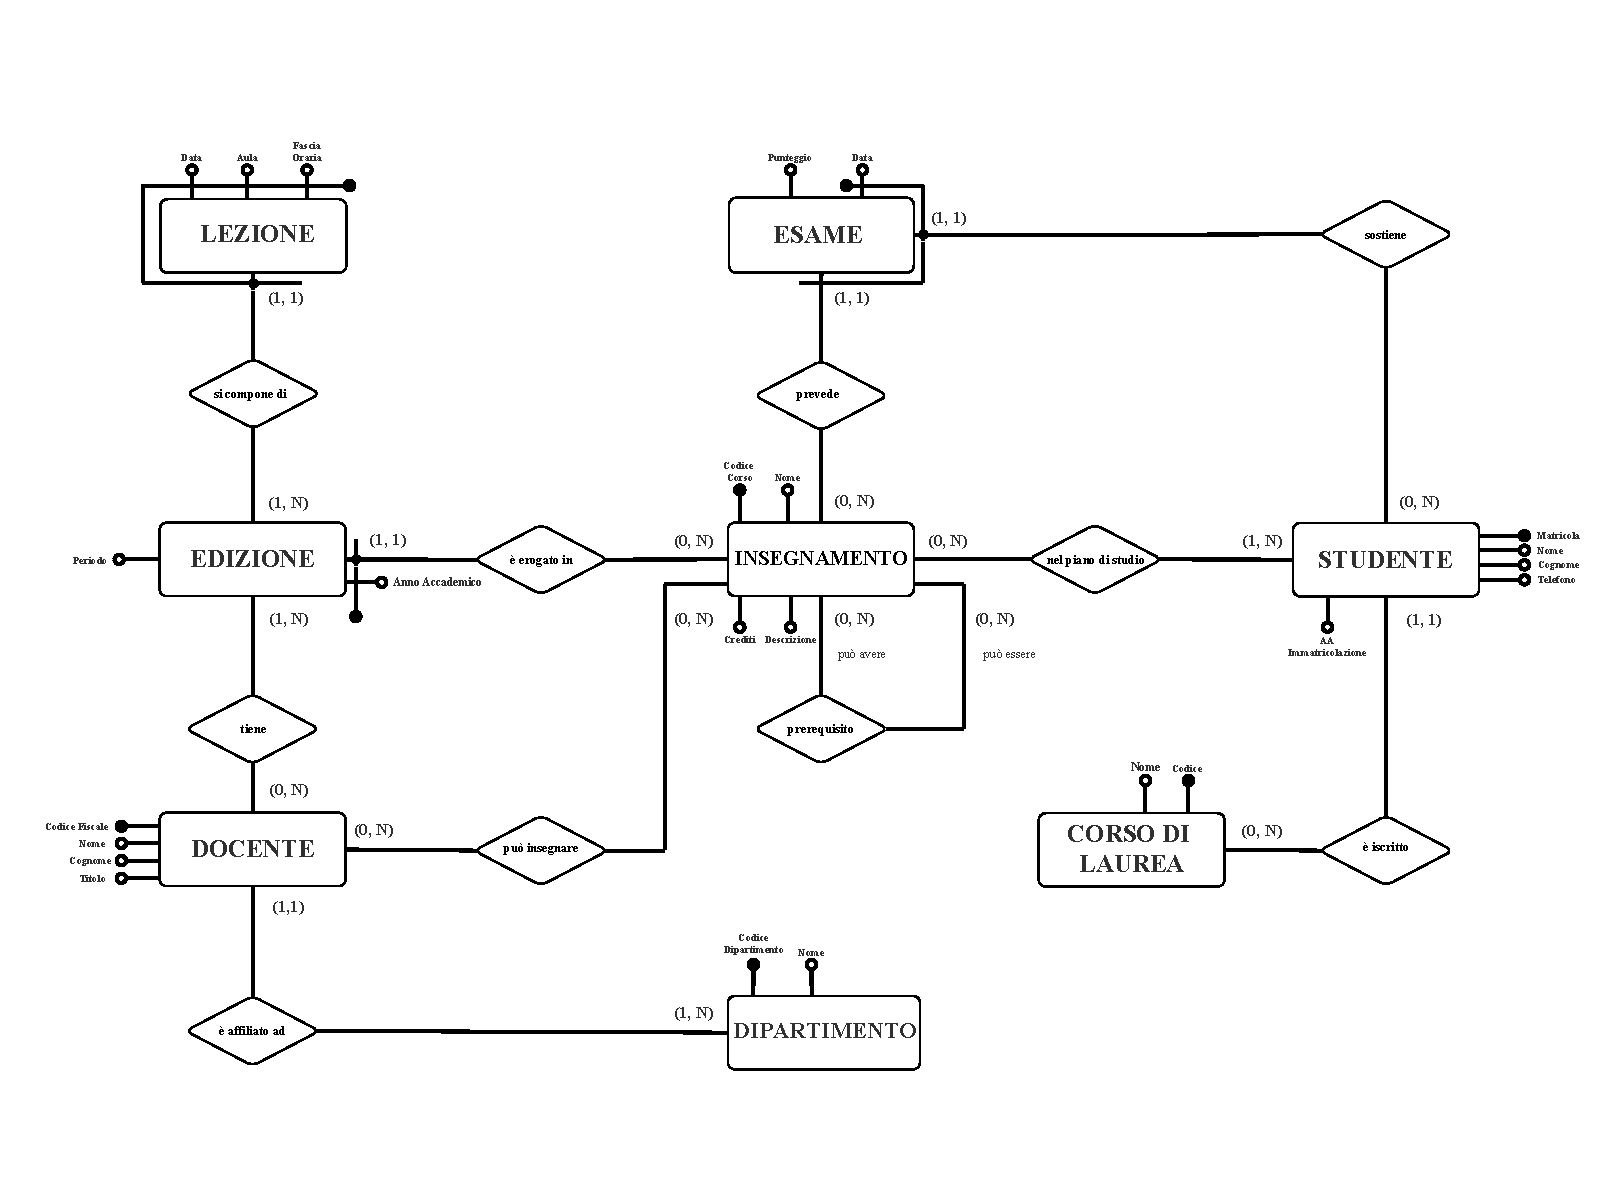
\includegraphics[width=\textwidth]{img/er.pdf}
    \caption{Schema ER per la gestione della didattica.}
    \label{fig:er_schema}
\end{figure}

\section{Vincoli di integrità e di dominio}
\label{sec:vincoli-di-integrita-e-di-dominio}

In questa sezione vengono descritte le regole che non si possono esprimere direttamente attraverso lo schema concettuale, ma che sono fondamentali per garantire che il sistema rispetti le regole della facoltà.

\subsection{Vincoli di propedeuticità}
\label{ssec:vincoli-di-propedeuticita}

\paragraph{Regola di precedenza degli esami}
Uno studente può registrare il superamento di una prova d'esame relativa a un insegnamento $I$ solo se risulta già certificato, per la medesima matricola, il superamento di tutti gli insegnamenti definiti come prerequisiti per $I$. In questo modo viene garantito il rispetto del corretto ordine di avanzamento della carriera.

\subsection{Vincoli temporali e di assegnazione}
\label{ssec:vincoli-temporali-e-di-assegnazione}

\paragraph{Unicità dell'edizione annuale}
Per ogni insegnamento presente nell'offerta formativa, non può essere attivata più di un'edizione nel medesimo anno accademico.
Questo garantisce che la pianificazione didattica sia univoca su base annuale.

\paragraph{Vincolo di abilitazione alla docenza}
Un docente può assumere la titolarità di un'edizione solo se risulta formalmente abilitato a tenere quello specifico insegnamento.
Tale regola impedisce l'assegnazione di incarichi didattici al di fuori delle competenze certificate dalla facoltà.

\subsection{Specifiche sui domini dei dati}
\label{ssec:specifiche-sui-domini-dei-dati}

\paragraph{Restrizioni sui periodi didattici}
L'organizzazione temporale della didattica su scala annuale è soggetta a parametri rigidi imposti dalla facoltà. Nello specifico, il periodo didattico in cui si svolge un'edizione deve necessariamente appartenere all'insieme finito $\{1, 2, 3\}$.

\paragraph{Restrizioni sulle fasce orarie}
La collocazione giornaliera delle singole lezioni segue vincoli logistici altrettanto restrittivi.
Tale parametro è infatti strettamente limitato a quattro blocchi temporali predefiniti, identificati dai valori discreti $\{1, 2, 3, 4\}$.

\paragraph{Restrizioni sui giorni di lezione}
Per garantire la coerenza del calendario didattico, la programmazione settimanale esclude i fine settimana.
Di conseguenza, il valore relativo al giorno in cui si svolge una lezione è rigorosamente limitato all'insieme testuale \{Lunedì, Martedì, Mercoledì, Giovedì, Venerdì\}.

\paragraph{Restrizioni sul titolo accademico}
Mentre il dipartimento di afferenza è gestito tramite un'entità dedicata, il titolo del docente è modellato come un dominio vincolato. Questa scelta dipende dalla natura statica del dato, che cambia molto raramente nel tempo. Il titolo deve quindi appartenere a un elenco chiuso di valori, come $\{Ricercatore, Professore Associato, Professore Ordinario\}$.


    \chapter{Progettazione logica}
    \section{Ristrutturazione dello Schema}
\label{sec:ristrutturazione-dello-schema}

\subsection{Analisi delle prestazioni}
\label{ssec:analisi-delle-prestazioni}

La tabella dei volumi costituisce lo strumento fondamentale per valutare i costi delle operazioni e analizzare le ridondanze, ponendo le basi per la corretta ristrutturazione dello schema ER.
Al suo interno vengono stimate le occorrenze previste per ciascun concetto della base di dati, valutate in una condizione di utilizzo a regime del sistema.

\begin{table}[h]
    \centering
    \renewcommand{\arraystretch}{1.4}
    \begin{tabular}{lcr}
        \textbf{Concetto} & \textbf{Tipo} & \textbf{Volume} \\
        \hline
        Dipartimento & E & 8 \\

        Corso di laurea & E & 80 \\

        Docente & E & 700 \\

        Insegnamento & E & 1.200 \\

        Edizione & E & 6.000 \\

        Lezione & E & 120.000 \\

        Studente & E & 16.000 \\

        Esame & E & 320.000 \\

        è affiliato ad & R & 700 \\

        è iscritto & R & 16.000 \\

        nel piano di studio & R & 320.000 \\

        sostiene & R & 320.000 \\

        prevede & R & 320.000 \\

        prerequisito & R & 360 \\

        può insegnare & R & 3.500 \\

        è erogato in & R & 6.000 \\

        tiene & R & 7.000 \\

        si compone di & R & 120.000 \\

    \end{tabular}
    \caption{Tabella dei volumi}
    \label{tab:volumi}
\end{table}

La stima dei volumi presentata nella Tabella \ref{tab:volumi} prende come modello di riferimento la realtà accademica dell'Università degli Studi di Udine\footnote{\url{https://www.uniud.it/it/ateneo-uniud/ateneo-uniud/numeri-ateneo}}. Le grandezze fondamentali riflettono i dati pubblici dell'Ateneo, ai quali è stato applicato un leggero arrotondamento per semplificare l'analisi quantitativa (ad esempio, i corsi di laurea sono stati approssimati a 80).

A partire da questi valori di base per studenti, docenti, dipartimenti e insegnamenti, i volumi delle entità subordinate e delle associazioni sono stati derivati analiticamente ipotizzando un orizzonte temporale di conservazione dello storico pari a 5 anni accademici, necessario per coprire l'intero ciclo di studi degli iscritti.

Per le entità \textit{Edizione} e \textit{Lezione}, considerando lo storico di 5 anni, i 1.200 insegnamenti erogati annualmente generano 6.000 istanze per l'entità \textit{Edizione} e per la relazione \textit{è erogato in}. Assumendo una media di 20 appuntamenti per edizione, si ricavano $6000 \cdot 20 = 120000$ istanze per l'entità \textit{Lezione} e per la relazione \textit{si compone di}.

Riguardo alla relazione \textit{nel piano di studio}, si stima che uno studente inserisca in media 20 insegnamenti durante l'intera carriera accademica. Considerando 16.000 studenti attivi e storicizzati, si ottiene un volume complessivo di $320000$ tuple.

Valutando l'entità \textit{Esame} e le relazioni \textit{sostiene} e \textit{prevede}, l'orizzonte di 5 anni permette di tracciare le carriere complete. Ipotizzando che l'esito (positivo o negativo) registri in media 20 verbalizzazioni a studente lungo l'intero percorso, si genera un totale di $320000$ istanze.

Passando all'assegnazione dei docenti, si ipotizza che ogni professore o ricercatore sia abilitato a insegnare mediamente 5 materie afferenti al proprio settore disciplinare, portando la relazione \textit{può insegnare} a $700 \cdot 5 = 3500$ tuple. Per la relazione \textit{tiene}, includendo le possibili co-docenze accumulate nel quinquennio, si stimano 7.000 assegnazioni distribuite sulle $6000$ edizioni.

Infine, per la relazione ricorsiva \textit{prerequisito}, si ipotizza che all'interno di ciascuno degli 80 corsi di laurea vi siano in media 4 o 5 insegnamenti strettamente propedeutici, generando una stima complessiva e costante di 360 istanze.

\subsection{Analisi dei cicli}
\label{ssec:analisi-dei-cicli}

Prima di procedere alla traduzione dello schema concettuale nel modello logico,
viene effettuata una verifica strutturale del diagramma ER per
individuare eventuali percorsi ciclici.
In particolare, sono stati individuati due cicli principali,
successivamente analizzati per stabilire se costituissero ridondanze strutturali da eliminare
oppure cicli giustificati da mantenere mediante opportuni vincoli di integrità nel modello logico.

\paragraph{Ciclo 1:}
Il primo ciclo si instaura tra le entità \textit{STUDENTE} - \textit{INSEGNAMENTO} - \textit{ESAME} - \textit{STUDENTE}. \\

\noindent
È possibile collegare uno studente a un insegnamento tramite due percorsi distinti:

\begin{enumerate}
    \item Il percorso diretto tramite la relazione \textit{nel piano di studio}.
    \item Il percorso indiretto tramite le relazioni \textit{sostiene} e \textit{prevede}.
\end{enumerate}

\noindent
Il ciclo non rappresenta una ridondanza, perché i due percorsi descrivono informazioni diverse.
Il primo percorso relativo ai corsi seguiti dallo studente ha uno scopo programmatorio, in quanto indica le attività che lo studente ha scelto nel proprio percorso di studi.
Il secondo percorso legato agli esami sostenuti, invece, ha uno scopo storico, poiché registra le prove realmente effettuate e concluse.
Eliminare uno dei due percorsi comporterebbe una perdita di informazioni,
pertanto lo schema ER viene mantenuto invariato. \\

\noindent
\textbf{Vincolo di integrità (Ciclo 1):} La correlazione logica tra i
due percorsi impone che uno studente non possa sostenere l'esame di un
corso non presente nel proprio piano di studi. Tale vincolo non è
esprimibile tramite la struttura del modello ER e viene pertanto
demandato a un \textit{trigger}, che, prima di ogni inserimento nella
relazione \textit{sostiene}, verifica che il corso associato
all'esame risulti già presente nel piano di studi dello studente,
in caso contrario l'operazione viene rifiutata.

\paragraph{Ciclo 2:}
Il secondo ciclo si instaura tra le entità \textit{DOCENTE} - \textit{INSEGNAMENTO} - \textit{EDIZIONE} - \mbox{\textit{DOCENTE}}. \\

\noindent
Un docente risulta collegato a un insegnamento tramite:

\begin{enumerate}
    \item Il percorso diretto tramite la relazione \textit{può insegnare}.
    \item Il percorso indiretto tramite le relazioni \textit{tiene} ed \textit{è erogato in}.
\end{enumerate}

\noindent
Anche in questo caso il ciclo non costituisce ridondanza strutturale.
La relazione \textit{può insegnare} modella un'abilitazione statica,
indicando le materie afferenti al settore scientifico-disciplinare del docente,
indipendentemente dall'effettiva erogazione.
Il percorso indiretto modella invece l'incarico reale assegnato in una precisa edizione.
Essendo abilitazione e assegnazione due concetti temporalmente e funzionalmente separati,
lo schema ER viene mantenuto invariato. \\

\noindent
\textbf{Vincolo di integrità (Ciclo 2):} La correlazione logica tra i
due percorsi impone che un docente non possa essere assegnato
all'edizione di un corso per il quale non risulti abilitato.
Anche questo vincolo viene demandato a un \textit{trigger}, che, prima di
ogni inserimento nella relazione \textit{tiene},
verifica che il docente compaia nella relazione \textit{può insegnare}
per il corso corrispondente all'edizione, altrimenti l'operazione viene rifiutata.

\subsection{Analisi delle ridondanze}
\label{ssec:analisi-delle-ridondanze}

In questa fase della progettazione logica, si analizza l'impatto prestazionale
derivante dal mantenimento degli attributi ridondanti
del modello concettuale all'interno del modello logico.
L'unico caso riguarda l'attributo derivato \textit{Crediti Ottenuti} in \textit{STUDENTE},
il cui valore è calcolabile sommando i crediti degli insegnamenti
per i quali lo studente ha registrato un esame superato (punteggio $\geq 18$). \\

\noindent
Per valutare se il risparmio computazionale in lettura
giustifichi il sovraccarico in scrittura,
l'analisi si basa su una stima delle frequenze di accesso ai dati.
Nello specifico, le operazioni coinvolte nell'analisi sono:
\begin{itemize}
    \item \textbf{Lettura:} verifica del totale dei crediti conseguiti da uno studente.
    Stimando che ogni studente consulti il proprio stato
    carriera mediamente 3 volte l'anno (inizio semestre, pre-sessione, verifica laurea),
    si ottiene $16.000 \text{ studenti} \times 3 = 48.000 \approx 50.000$ esecuzioni/anno.
    \item \textbf{Scrittura:} aggiornamento dei crediti totali conseguiti da uno studente al superamento di un esame.
    Stimando 5 esami superati all'anno per studente, si ottiene
    $16.000 \text{ studenti} \times 5 = 80.000$ esecuzioni/anno.
\end{itemize}

\noindent
Per uniformare il confronto tra operazioni di natura diversa si adotta la convenzione $1w = 2r$ ,
ossia ogni accesso in scrittura equivale a due accessi in lettura,
esprimendo così il costo in letture equivalenti.

\subsubsection{Accessi in assenza della ridondanza}
\label{sssec:accessi-in-assenza-della-ridondanza}

In assenza dell'attributo ridondante, per calcolare il totale dei
crediti conseguiti da uno studente, il DBMS deve accedere a tutti
gli esami superati in \textit{ESAME} (in media 12 record per studente)
e, per ciascuno, recuperare il numero di crediti
dall'entità \textit{INSEGNAMENTO}, complessivamente
$12 \times 2 = 24$ accessi per esecuzione,
poiché ogni esame richiede una lettura in \textit{ESAME}
e una in \textit{INSEGNAMENTO}.
$$24 \text{ letture} \times 50.000 \text{ volte/anno} = 1.200.000 \text{ accessi in lettura/anno}$$
L'inserimento di un nuovo esame richiede la sola scrittura
di una tupla in \textit{ESAME}, ossia 2 accessi in lettura.
$$2 \text{ accessi} \times 80.000 \text{ volte/anno} = 160.000 \text{ accessi in lettura/anno}$$

\subsubsection{Accessi in presenza della ridondanza}
\label{sssec:accessi-in-presenza-della-ridondanza}

Mantenendo l'attributo ridondante,
la verifica del totale crediti si riduce a
un singolo accesso alla tupla dello studente, eliminando
completamente la navigazione tra \textit{ESAME} e
\textit{INSEGNAMENTO}.
$$1 \text{ lettura} \times 50.000 \text{ volte/anno} = 50.000 \text{ accessi in lettura/anno}$$
Al contrario, la scrittura si complica dato che oltre all'inserimento in \textit{ESAME}
(1 scrittura), se il punteggio è $\geq 18$, un trigger deve leggere
i crediti dell'insegnamento da \textit{INSEGNAMENTO} (1 lettura) e
aggiornare i crediti dello studente (1 lettura e 1 scrittura),
per un totale di 6 accessi considerando la conversione.
$$6 \text{ accessi} \times 80.000 = 480.000 \text{ accessi in lettura/anno}$$

\subsubsection{Decisione sulla ridondanza}
\label{sssec:decisione-sulla-ridondanza}

I costi complessivi annui espressi in accessi in lettura sono riassunti nella seguente tabella:

\begin{table}[h]
    \centering
    \renewcommand{\arraystretch}{1.2}
    \begin{tabular}{|l|r|r|}
        \hline
        \textbf{Operazione} & \textbf{Con ridondanza}
        & \textbf{Senza ridondanza} \\
        \hline
        Lettura & 50.000 & 1.200.000 \\
        \hline
        Scrittura & 480.000 & 160.000 \\
        \hline
        \textbf{Totale} & \textbf{530.000} & \textbf{1.360.000} \\
        \hline
    \end{tabular}
    \caption{Bilancio accessi equivalenti per \textit{Crediti Ottenuti}}
\end{table}

\noindent
L'analisi evidenzia un vantaggio netto nel mantenere la ridondanza.
L'abbattimento del 96\% dei costi di lettura (da 1.200.000 a 50.000 accessi/anno)
compensa ampiamente il sovraccarico in scrittura (+320.000 accessi).
Con un bilancio complessivo ridotto da 1.360.000 a 530.000 accessi annui,
viene scelto di mantenere \textit{Crediti Ottenuti} in \textit{STUDENTE}.
La sua coerenza sarà garantita da un trigger
attivato ad ogni inserimento in \textit{ESAME} con punteggio
$\geq 18$, la cui implementazione è descritta nella sezione di
progettazione fisica.


    \section{Progettazione Logica}

\subsection{Tabella dei volumi}

Per valutare i costi delle operazioni, per effettuare una corretta analisi delle ridondanze 
e quindi per effettuare una corretta ristrutturazione dello schema E-R, 
si rende necessaria una tabella dei volumi in cui per ogni oggetto stimiamo 
la sua quantità media presente nella base di dati a metà del suo ciclo di vita operativo.

\begin{table}[h]
    \centering
    \renewcommand{\arraystretch}{1.2}
    \begin{tabular}{|l|c|r|}
        \hline
        \textbf{Concetto} & \textbf{Tipo} & \textbf{Volume} \\
        \hline
        DIPARTIMENTO & E & 3 \\
        \hline
        CORSO DI LAUREA & E & 21 \\
        \hline
        DOCENTE & E & 320 \\
        \hline
        CORSO & E & 350 \\
        \hline
        EDIZIONE & E & 700 \\
        \hline
        LEZIONE & E & 14.000 \\
        \hline
        STUDENTE & E & 6.500 \\
        \hline
        ESAME & E & 78.000 \\
        \hline
        è affiliato ad & R & 320 \\
        \hline
        è iscritto & R & 6.500 \\
        \hline
        nel piano di studio & R & 130.000 \\
        \hline
        sostiene & R & 78.000 \\
        \hline
        prevede & R & 78.000 \\
        \hline
        prerequisito & R & 100 \\
        \hline
        può insegnare & R & 960 \\
        \hline
        è erogato in & R & 700 \\
        \hline
        tiene & R & 850 \\
        \hline
        si compone di & R & 14.000 \\
        \hline
    \end{tabular}
    \caption{Tabella dei volumi stimati per il Polo Scientifico}
    \label{tab:volumi}
\end{table}

\noindent 
La stima dei volumi (Tabella \ref{tab:volumi}) è stata ricavata da un'analisi quantitativa legata a una realtà accademica concreta, 
prendendo come modello di riferimento i tre dipartimenti del Polo Scientifico dell'Università degli Studi di Udine (\texttt{DMIF}, \texttt{DPIA}, \texttt{DI4A}). 
I dati di riferimento sono stati estrapolati e proporzionati partendo dagli Open Data ufficiali del Ministero dell'Università e della Ricerca (portale USTAT) 
relativi all'anno 2024 e dall'offerta formativa di ateneo per l'anno accademico 2023/2024. 
Sapendo che l'università ospita storicamente circa 16.000 iscritti complessivi e che l'area STEM (Informatica, Ingegneria, Scienze Agrarie) 
assorbe tipicamente il 40\% del totale degli iscritti, si è stimato un volume di circa 6.500 studenti attivi. 
Allo stesso modo, l'organico di docenti strutturati afferenti a questi tre dipartimenti ammonta a circa 320 unità, 
i quali gestiscono un'offerta di 21 corsi di laurea (tra triennali e magistrali) e 350 insegnamenti unici. \\

\noindent
Partendo da queste basi fattuali, i volumi delle relazioni e delle entità intermedie sono stati ricavati matematicamente per un sistema a metà del suo ciclo di vita:

\begin{itemize}
    \item \textbf{EDIZIONE e LEZIONE}: Mantenendo uno storico operativo di due anni accademici, i 350 corsi generano 700 istanze per l'entità EDIZIONE e per la relazione \textit{è erogato in}. Assumendo una media di 20 appuntamenti per edizione, si ricavano $700 \cdot 20 = 14.000$ istanze per l'entità LEZIONE e per la relazione \textit{si compone di}.
    \item \textbf{Piano di studio}: Si stima che uno studente inserisca in media 20 corsi nel proprio piano di studi durante la sua carriera. Considerando 6.500 studenti attivi, la relazione \textit{nel piano di studio} conta $6.500 \cdot 20 = 130.000$ tuple.
    \item \textbf{ESAME, sostiene e prevede}: Considerando l'eterogeneità della popolazione studentesca, costituita da neo-immatricolati, studenti in pari e fuori corso, si stima una media ponderata di 12 esami superati per studente. Di conseguenza, l'entità ESAME e le relazioni \textit{sostiene} e \textit{prevede} generano 6.500 $\cdot$ 12 = 78.000 istanze.
    \item \textbf{può insegnare e tiene}: Ipotizzando che ogni docente sia abilitato a insegnare mediamente 3 corsi afferenti al proprio settore disciplinare, la relazione \textit{può insegnare} genera $320 \cdot 3 = 960$ tuple. Per la relazione \textit{tiene}, includendo le co-docenze, si stimano 850 assegnazioni sulle 700 edizioni attive.
    \item \textbf{prerequisito}: Si ipotizza che all'interno di ciascuno dei 21 corsi di laurea vi siano in media 4 o 5 esami propedeutici per poter essere sostenuti, generando una stima di 100 istanze per la relazione ricorsiva.
\end{itemize}

\subsection{Analisi delle ridondanze}

In questa sezione viene valutata l'opportunità di introdurre una ridondanza controllata all'interno dello schema logico. 
Si evidenzia che lo schema concettuale Entità-Relazioni (E-R) precedentemente definito è rigorosamente privo di ridondanze, 
tutte le entità in esso presenti contengono esclusivamente attributi atomici e non derivabili. 
In questa fase di progettazione logica, tuttavia, si analizza l'impatto prestazionale derivante dall'introduzione intenzionale di un attributo ridondante, 
denominato \textit{NumeroIscritti}, all'interno di \textit{CORSO}. \\ 

\noindent
Tale scelta comporta una denormalizzazione del modello, poiché l'informazione legata al numero di studenti 
che hanno scelto un determinato insegnamento è già interamente ricavabile in modo dinamico contando le tuple della relazione \textit{nel piano di studio}. 
L'obiettivo dell'analisi è stabilire se il risparmio computazionale in lettura giustifichi il sovraccarico in scrittura e la potenziale complessità di gestione delle anomalie di modifica. \\

\noindent 
I due task principali selezionati per valutare l'impatto di questa modifica sono:
\begin{itemize}
    \item \textbf{Task 1 (Calcolo iscritti a un corso specifico)}: Dato un corso $X$, restituire il numero totale di studenti che lo hanno inserito nel proprio piano di studi (corrisponde all'OPERAZIONE 1).
    \item \textbf{Task 2 (Inserimento di un corso nel piano di studi)}: Dato un corso $X$, inserirlo nel piano di studi di un determinato studente (corrisponde all'OPERAZIONE 4).
\end{itemize}

\noindent 
In base ai parametri dimensionali stabiliti, si stima che il Task 1 venga eseguito con una frequenza di 20.000 volte all'anno da parte di docenti e segreterie per il monitoraggio delle classi. 
Il Task 2 viene eseguito interattivamente dagli studenti principalmente a ridosso dell'inizio dei semestri, registrando circa 32.500 modifiche annue ($6.500 \text{ studenti} \cdot 5 \text{ corsi/anno}$).

\subsubsection{Accessi in assenza della ridondanza}

\paragraph{Task 1:} In assenza dell'attributo ridondante, per contare gli iscritti a un corso $X$, il DBMS deve scansionare la relazione \textit{nel piano di studio}. Avendo stimato un volume totale di 130.000 tuple distribuite su 350 corsi, l'operazione richiede mediamente l'accesso in lettura a $130.000 / 350 \approx 371$ record per ogni interrogazione.
$$371 \text{ letture} \cdot 20.000 \text{ volte/anno} = 7.420.000 \text{ accessi in lettura all'anno}$$

\paragraph{Task 2:} L'inserimento del corso richiede esclusivamente la scrittura di una nuova tupla all'interno della relazione \textit{nel piano di studio}, senza impattare altre strutture.
$$1 \text{ scrittura} \cdot 32.500 \text{ volte/anno} = 32.500 \text{ accessi in scrittura all'anno}$$

\subsubsection{Accessi in presenza della ridondanza}

\paragraph{Task 1:} Introducendo l'attributo ridondante, il sistema non deve più navigare nella relazione intermedia ed è sufficiente accedere alla singola istanza dell'entità \textit{CORSO} corrispondente all'insegnamento $X$ e leggerne direttamente il valore memorizzato.
$$1 \text{ lettura} \cdot 20.000 \text{ volte/anno} = 20.000 \text{ accessi in lettura all'anno}$$

\paragraph{Task 2:} In presenza di ridondanza, l'operazione di scrittura si complica. Oltre all'inserimento del record nella relazione \textit{nel piano di studio} (1 scrittura), il sistema deve aggiornare il contatore nell'entità \textit{CORSO}, richiedendo una lettura preliminare del valore corrente e la successiva riscrittura del dato incrementato (1 lettura e 1 scrittura). Ogni esecuzione comporta quindi 1 lettura e 2 scritture complessive.
$$32.500 \text{ letture/anno e } 65.000 \text{ scritture/anno}$$

\subsubsection{Decisione sulla ridondanza}

Al fine di confrontare in modo omogeneo i due scenari, le operazioni di modifica vengono pesate con un costo computazionale doppio rispetto alle operazioni di consultazione ($1w = 2r$). 
I costi complessivi annui espressi in accessi equivalenti in lettura sono riassunti nella seguente tabella:

\begin{table}[h]
    \centering
    \renewcommand{\arraystretch}{1.2}
    \begin{tabular}{|l|r|r|}
        \hline
        \textbf{Task} & \textbf{Con ridondanza} & \textbf{Senza ridondanza} \\
        \hline
        Task 1 & 20.000 & 7.420.000 \\
        \hline
        Task 2 & 162.500 & 65.000 \\
        \hline
        \textbf{Totale [Accessi equivalenti]} & \textbf{182.500} & \textbf{7.485.000} \\
        \hline
    \end{tabular}
    \caption{Bilancio complessivo degli accessi}
\end{table}

\noindent
Il bilancio dei costi evidenzia un divario macroscopico, a fronte di un incremento controllato dei costi di scrittura per il Task 2 (+97.500 accessi equivalenti), 
il Task 1 beneficia di un abbattimento drastico dei tempi di risposta, consentendo di risparmiare oltre 7,3 milioni di accessi annui sul disco. \\

\noindent 
Dal punto di vista progettuale, si decide pertanto di accettare il compromesso della denormalizzazione, modificando formalmente lo schema logico rispetto a quello concettuale originario. 
L'attributo ridondante \textit{NumeroIscritti} viene ufficialmente introdotto all'interno dell'entità \textit{CORSO}, 
delegando a opportuni vincoli di integrità a livello logico (tramite trigger in fase di implementazione) il compito di mantenere aggiornato il contatore ed evitare qualsiasi rischio di inconsistenza della base di dati.

\subsubsection{Analisi dei cicli}

L'analisi delle ridondanze si è estesa alla verifica strutturale dello schema concettuale per l'individuazione di eventuali cicli. 
All'interno del diagramma E-R sono stati individuati due percorsi ciclici principali, i quali sono stati analizzati per determinare la presenza di derivabilità.

\paragraph{Ciclo 1:}
Il primo ciclo si instaura tra le entità \textit{STUDENTE}, \textit{CORSO} ed \textit{ESAME}. È possibile collegare uno studente a un corso tramite due percorsi distinti:

\begin{enumerate}
    \item L'associazione diretta tramite la relazione \textit{nel piano di studio}.
    \item La navigazione indiretta tramite le relazioni \textit{sostiene} e \textit{prevede}.
\end{enumerate}

\noindent
Il ciclo \textbf{non rappresenta una ridondanza}, perché i due percorsi descrivono informazioni diverse.
La relazione relativa ai corsi seguiti dallo studente ha uno scopo programmatorio, in quanto indica le attività che lo studente ha scelto nel proprio percorso di studi.
La relazione legata agli esami sostenuti, invece, ha uno scopo storico, poiché registra le prove realmente effettuate e concluse.
Di conseguenza, eliminare una delle due relazioni comporterebbe la perdita di informazioni importanti.
La coerenza tra i due percorsi, ad esempio il fatto che uno studente possa sostenere solo esami relativi a corsi presenti nel proprio piano di studi, 
viene garantita tramite un vincolo di integrità implementato con un trigger, e non attraverso modifiche alla struttura dello schema.

\paragraph{Ciclo 2:}
Il secondo ciclo si instaura tra le entità \textit{DOCENTE}, \textit{CORSO} ed \textit{EDIZIONE}. Un docente risulta collegato a un corso tramite:

\begin{enumerate}
    \item L'associazione diretta tramite la relazione \textit{può insegnare}.
    \item La navigazione indiretta tramite le relazioni \textit{tiene} ed \textit{è erogato in}.
\end{enumerate}

\noindent
Anche in questo caso il ciclo \textbf{non costituisce ridondanza}. 
La relazione \textit{può insegnare} modella un'abilitazione di base, indicando le materie afferenti al settore scientifico-disciplinare del docente, 
indipendentemente dall'effettiva erogazione. Il percorso indiretto modella invece l'incarico reale assegnato in un preciso anno accademico. 
Essendo l'abilitazione (statica) e l'assegnazione (dinamica) due concetti temporalmente e funzionalmente separati, si decide di mantenere intatto lo schema E-R.

\subsection{Schema Logico}
Di seguito si riporta lo schema logico risultante. Per convenzione, gli attributi che compongono la \underline{chiave primaria} sono sottolineati, mentre le chiavi esterne sono contrassegnate da un asterisco (*).

\begin{itemize}
    \item \textbf{DIPARTIMENTO} (\underline{CodiceDipartimento}, Nome)
    \item \textbf{CORSO\_DI\_LAUREA} (\underline{CodiceCDL}, Nome)
    \item \textbf{DOCENTE} (\underline{CodiceFiscale}, Nome, Cognome, Titolo, CodiceDipartimento*)
    \item \textbf{STUDENTE} (\underline{Matricola}, Nome, Cognome, Telefono, AA\_Immatricolazione, CodiceCDL*)
    \item \textbf{CORSO} (\underline{CodiceCorso}, Nome, Crediti, Descrizione, NumeroIscritti)
    \item \textbf{EDIZIONE} (\underline{CodiceCorso*}, \underline{AnnoAccademico}, \underline{Periodo})
    \item \textbf{LEZIONE} (\underline{CodiceCorso*}, \underline{AnnoAccademico*}, \underline{Periodo*}, \underline{Data}, \underline{FasciaOraria}, Aula)
    \item \textbf{ESAME} (\underline{Matricola*}, \underline{CodiceCorso*}, \underline{Data}, Punteggio)
    \item \textbf{PIANO\_DI\_STUDIO} (\underline{Matricola*}, \underline{CodiceCorso*})
    \item \textbf{PREREQUISITO} (\underline{CodiceCorsoPropedeutico*}, \underline{CodiceCorsoSuccessivo*})
    \item \textbf{PUO\_INSEGNARE} (\underline{CodiceFiscale*}, \underline{CodiceCorso*})
    \item \textbf{TIENE} (\underline{CodiceFiscale*}, \underline{CodiceCorso*}, \underline{AnnoAccademico*}, \underline{Periodo*})
\end{itemize}

\subsection{Vincoli di Integrità Referenziale}
Per garantire la coerenza della base di dati, si definiscono esplicitamente i seguenti vincoli di integrità referenziale (Foreign Keys) per lo schema logico appena descritto:

\begin{itemize}
    \item \textbf{DOCENTE}.CodiceDipartimento $\rightarrow$ \textbf{DIPARTIMENTO}.CodiceDipartimento
    \item \textbf{STUDENTE}.CodiceCDL $\rightarrow$ \textbf{CORSO\_DI\_LAUREA}.CodiceCDL
    \item \textbf{EDIZIONE}.CodiceCorso $\rightarrow$ \textbf{CORSO}.CodiceCorso
    \item \textbf{LEZIONE}.(CodiceCorso, AnnoAccademico, Periodo) $\rightarrow$ \textbf{EDIZIONE}.(CodiceCorso, AnnoAccademico, Periodo)
    \item \textbf{ESAME}.Matricola $\rightarrow$ \textbf{STUDENTE}.Matricola
    \item \textbf{ESAME}.CodiceCorso $\rightarrow$ \textbf{CORSO}.CodiceCorso
    \item \textbf{PIANO\_DI\_STUDIO}.Matricola $\rightarrow$ \textbf{STUDENTE}.Matricola
    \item \textbf{PIANO\_DI\_STUDIO}.CodiceCorso $\rightarrow$ \textbf{CORSO}.CodiceCorso
    \item \textbf{PREREQUISITO}.CodiceCorsoPropedeutico $\rightarrow$ \textbf{CORSO}.CodiceCorso
    \item \textbf{PREREQUISITO}.CodiceCorsoSuccessivo $\rightarrow$ \textbf{CORSO}.CodiceCorso
    \item \textbf{PUO\_INSEGNARE}.CodiceFiscale $\rightarrow$ \textbf{DOCENTE}.CodiceFiscale
    \item \textbf{PUO\_INSEGNARE}.CodiceCorso $\rightarrow$ \textbf{CORSO}.CodiceCorso
    \item \textbf{TIENE}.CodiceFiscale $\rightarrow$ \textbf{DOCENTE}.CodiceFiscale
    \item \textbf{TIENE}.(CodiceCorso, AnnoAccademico, Periodo) $\rightarrow$ \textbf{EDIZIONE}.(CodiceCorso, AnnoAccademico, Periodo)
\end{itemize}


    \chapter{Progettazione fisica}
    \section{Progettazione Fisica e Script SQL}
\label{sec:progettazione-fisica-e-script-sql}

    \chapter{Operazioni e interrogazioni}
    \section{Interrogazioni di Test}
\label{sec:interrogazioni-di-test}


    \appendix
    \chapter{Glossario}
    \renewcommand{\arraystretch}{1.4}
\begin{longtable}{ >{\raggedright\arraybackslash}p{3.5cm} >{\raggedright\arraybackslash}p{7.5cm} >{\raggedright\arraybackslash}p{3.5cm}}


    \hline
    \textbf{Termine} & \textbf{Descrizione} & \textbf{Termini correlati} \\
    \hline
    \endfirsthead

    \hline
    \textbf{Termine} & \textbf{Descrizione} & \textbf{Termini correlati} \\
    \hline
    \endhead

    \hline
    \multicolumn{3}{r}{{Continua nella pagina successiva}} \\
    \endfoot

    \hline
    \caption{Glossario} \label{tab:glossario}
    \endlastfoot

    \textbf{Insegnamento} & Corso universitario identificato da un codice e caratterizzato da crediti, descrizione e prerequisiti. & Edizione, Prerequisito, Piano di studio \\

    \textbf{Edizione} & Erogazione di un insegnamento in un determinato anno accademico e periodo didattico. Può essere tenuta da uno o più docenti. & Insegnamento, Docente, Lezione \\

    \textbf{Lezione} & Singolo appuntamento all'interno del calendario settimanale di un'edizione. È identificata univocamente dalla terna giorno, fascia oraria e aula. & Edizione \\

    \textbf{Prerequisito} & Insegnamento da superare prima di poter sostenere l'esame di un altro insegnamento. & Insegnamento \\

    \textbf{Studente} & Persona iscritta all'università, identificata dal numero di matricola, associata a un unico corso di laurea. & Piano di studio, Esame, Corso di Laurea \\

    \textbf{Piano di studio} & Insieme dei corsi scelti dallo studente per il proprio percorso accademico. & Studente, Insegnamento \\

    \textbf{Esame} & Tentativo sostenuto da uno studente per un determinato insegnamento, costituito da un'unica prova d'esame. Memorizza il punteggio ottenuto, inclusi i voti insufficienti (< 18). & Studente, Insegnamento \\

    \textbf{Docente} & Figura accademica afferente a un dipartimento, abilitata all'insegnamento. & Edizione, Insegnamento, Dipartimento \\

    \textbf{Corso di Laurea} & Percorso di studi specifico frequentato dallo studente (es. Informatica triennale). & Studente \\

    \textbf{Dipartimento} & Struttura accademica di afferenza per i docenti (es. Dipartimento di Scienze Matematiche, Informatiche e Fisiche). & Docente \\

\end{longtable}
\end{document}